% =====================================================================
\chapter{Convexidad}
\label{tema:5}
% =====================================================================

En una función convexa, todo mínimo local es global, de modo que un método de descenso no puede quedar atrapado en un mínimo malo. Este tema define los conjuntos y las funciones convexas, demuestra las caracterizaciones de primer y segundo orden, establece las operaciones que conservan la convexidad y las aplica a la entropía cruzada. Termina explicando por qué la pérdida de una red profunda no es convexa. Se sigue~\cite[§3.1, §3.2 y §4.2]{bv} y las transparencias correspondientes de~\cite{ee364a}.

\section{Conjuntos y funciones convexas}

\begin{definicion}[Conjunto convexo]
Un conjunto $C\subseteq\R^{n}$ es \emph{convexo} si, para todo $a,b\in C$ y todo $\lambda\in[0,1]$, el punto $\lambda a+(1-\lambda)b$ pertenece a $C$: contiene el segmento que une dos cualesquiera de sus puntos.
\end{definicion}

\begin{definicion}[Función convexa]\label{def:convexa}
Sea $C\subseteq\R^{n}$ convexo. Una función $f\colon C\to\R$ es \emph{convexa} si
\[
f\bigl(\lambda a+(1-\lambda)b\bigr)\le\lambda f(a)+(1-\lambda)f(b)\qquad\text{para todo } a,b\in C,\ \lambda\in[0,1],
\]
y \emph{estrictamente convexa} si la desigualdad es estricta cuando $a\ne b$ y $\lambda\in(0,1)$. Se dice que $f$ es \emph{cóncava} si $-f$ es convexa.
\end{definicion}

Geométricamente, la cuerda que une $(a,f(a))$ con $(b,f(b))$ queda por encima de la gráfica (\cref{fig:convexa}). Son convexas, por ejemplo, las funciones afines $a\T x+b$ (con igualdad en la definición), toda norma (por la desigualdad triangular y la homogeneidad) y $x\mapsto e^{x}$ en $\R$.

\begin{figure}[h]
\centering
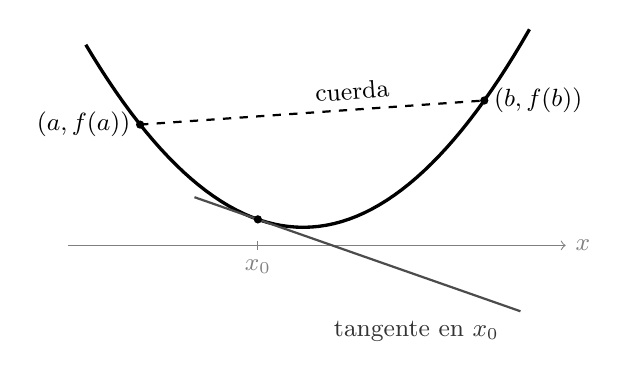
\begin{tikzpicture}[scale=1.15,font=\small,declare function={f(\x)=0.35*\x*\x+0.2;}]
  \draw[->,gray] (-2.6,0) -- (2.9,0) node[right] {$x$};
  \draw[very thick,domain=-2.4:2.5,samples=60] plot (\x,{f(\x)});
  \coordinate (A) at (-1.8,{f(-1.8)});
  \coordinate (B) at (2,{f(2)});
  \fill (A) circle (1.3pt) node[left] {$(a,f(a))$};
  \fill (B) circle (1.3pt) node[right] {$(b,f(b))$};
  \draw[thick,dashed] (A) -- (B) node[pos=0.62,above,sloped] {cuerda};
  \draw[thick,gray!60!black,domain=-1.2:2.4] plot (\x,{f(-0.5)+0.7*(-0.5)*(\x+0.5)});
  \fill (-0.5,{f(-0.5)}) circle (1.3pt);
  \node[gray!40!black] at (1.25,-0.95) {tangente en $x_0$};
  \draw[gray] (-0.5,0.05) -- (-0.5,-0.05) node[below] {$x_0$};
\end{tikzpicture}
\caption{Una función convexa queda por debajo de sus cuerdas (\cref{def:convexa}) y por encima de sus tangentes (\cref{teo:primer-orden}).}
\label{fig:convexa}
\end{figure}

\begin{lema}[Restricción a rectas]\label{lem:rectas}
Sea $C$ abierto y convexo. Una función $f\colon C\to\R$ es convexa si y solo si, para todo $x\in C$ y todo $v\in\R^{n}$, la función de una variable $\varphi(t)=f(x+tv)$ es convexa en el intervalo $\{t:x+tv\in C\}$.
\end{lema}

\begin{proof}
Si $f$ es convexa, para $t_1,t_2$ en el intervalo, $\varphi(\lambda t_1+(1-\lambda)t_2)=f\bigl(\lambda(x+t_1v)+(1-\lambda)(x+t_2v)\bigr)\le\lambda\varphi(t_1)+(1-\lambda)\varphi(t_2)$. Recíprocamente, dados $a,b\in C$, se toma $x=b$, $v=a-b$: entonces $\varphi(\lambda)=f(\lambda a+(1-\lambda)b)$ y la convexidad de $\varphi$ entre $t=0$ y $t=1$ es exactamente la desigualdad de la \cref{def:convexa}.
\end{proof}

\section{Condiciones de primer y segundo orden}

\begin{teorema}[Condición de primer orden]\label{teo:primer-orden}
Sea $C$ abierto y convexo y $f\colon C\to\R$ diferenciable. Entonces $f$ es convexa si y solo si
\[
f(b)\ge f(a)+\nabla f(a)\T(b-a)\qquad\text{para todo } a,b\in C.
\]
\end{teorema}

\begin{proof}
($\Rightarrow$) Para $\lambda\in(0,1]$, la convexidad da $f(a+\lambda(b-a))\le f(a)+\lambda\bigl(f(b)-f(a)\bigr)$, es decir,
\[
\frac{f(a+\lambda(b-a))-f(a)}{\lambda}\le f(b)-f(a).
\]
Cuando $\lambda\to 0^{+}$, el miembro izquierdo tiende a $\nabla f(a)\T(b-a)$ (\cref{prop:direccional}, sin normalizar la dirección), y se obtiene la desigualdad.

($\Leftarrow$) Sean $a,b\in C$, $\lambda\in[0,1]$ y $m=\lambda a+(1-\lambda)b$. Aplicando la hipótesis en el punto $m$ hacia $a$ y hacia $b$,
\[
f(a)\ge f(m)+\nabla f(m)\T(a-m),\qquad f(b)\ge f(m)+\nabla f(m)\T(b-m).
\]
Multiplicando por $\lambda$ y $1-\lambda$ y sumando, el término del gradiente se anula, porque $\lambda(a-m)+(1-\lambda)(b-m)=0$, y queda $\lambda f(a)+(1-\lambda)f(b)\ge f(m)$.
\end{proof}

La condición de primer orden dice que el plano tangente en cualquier punto es una cota inferior global de $f$: la información local del gradiente proporciona información global.

\begin{teorema}[Condición de segundo orden]\label{teo:segundo-orden}
Sea $C$ abierto y convexo y $f\in C^{2}(C)$. Entonces $f$ es convexa si y solo si $H_f(x)\succeq 0$ para todo $x\in C$. Si $H_f(x)\succ 0$ para todo $x\in C$, entonces $f$ es estrictamente convexa.
\end{teorema}

\begin{proof}
($\Leftarrow$) Sean $a,b\in C$. Por el \cref{teo:taylor}(i), $f(b)=f(a)+\nabla f(a)\T(b-a)+\tfrac12(b-a)\T H_f(\xi)(b-a)$ para un punto $\xi$ del segmento, que está en $C$. El último término es $\ge 0$, luego se cumple la condición de primer orden y $f$ es convexa por el \cref{teo:primer-orden}. Si $H_f\succ 0$ y $a\ne b$, el término es $>0$; repitiendo la demostración del \cref{teo:primer-orden} con desigualdades estrictas se obtiene la convexidad estricta.

($\Rightarrow$) Supóngase que existen $x\in C$ y $v$ con $v\T H_f(x)v<0$, y sea $\varphi(t)=f(x+tv)$. Por la demostración del \cref{teo:taylor}, $\varphi''(0)=v\T H_f(x)v<0$ y, por continuidad, $\varphi''<0$ en un intervalo alrededor de $0$. En ese intervalo $\varphi$ es estrictamente cóncava, luego no es convexa, y por el \cref{lem:rectas} tampoco lo es $f$.
\end{proof}

\begin{ejemplo}\label{ej:cuad-convexa}
$f(x,y)=x^{2}+xy+y^{2}$ tiene hessiano constante $\begin{pmatrix}2&1\\1&2\end{pmatrix}$, con autovalores~1 y~3. Por el \cref{teo:segundo-orden}, es estrictamente convexa en $\R^{2}$. En cambio, $x^{2}-y^{2}$, con autovalores $2$ y $-2$, no es convexa.
\end{ejemplo}

\begin{observacion}
El recíproco de la segunda parte del \cref{teo:segundo-orden} es falso: $f(x)=x^{4}$ es estrictamente convexa en $\R$, pero $f''(0)=0$.
\end{observacion}

\section{Mínimos de funciones convexas}

\begin{teorema}[Mínimos locales y globales]\label{teo:local-global}
Sea $f\colon C\to\R$ convexa. Todo mínimo local de $f$ es un mínimo global. Si además $f$ es diferenciable y $C$ es abierto, un punto $x^{*}$ es mínimo global si y solo si $\nabla f(x^{*})=0$.
\end{teorema}

\begin{proof}
Sea $x^{*}$ un mínimo local, con $f(x)\ge f(x^{*})$ si $\norm{x-x^{*}}<r$, y supóngase que existe $b\in C$ con $f(b)<f(x^{*})$. Para $\lambda\in(0,1)$ suficientemente pequeño, el punto $m=(1-\lambda)x^{*}+\lambda b$ está a distancia $\lambda\norm{b-x^{*}}<r$ de $x^{*}$, y por convexidad
\[
f(m)\le(1-\lambda)f(x^{*})+\lambda f(b)<f(x^{*}),
\]
lo que contradice que $x^{*}$ sea mínimo local. Para la segunda afirmación: si $x^{*}$ es mínimo, $\nabla f(x^{*})=0$ por el \cref{teo:fermat}; si $\nabla f(x^{*})=0$, el \cref{teo:primer-orden} da $f(b)\ge f(x^{*})$ para todo $b\in C$.
\end{proof}

Para funciones no convexas, $\nabla f=0$ solo es una condición necesaria. Para funciones convexas es también suficiente, y además global. Por eso el descenso de gradiente con una tasa adecuada resuelve los problemas convexos, como la regresión lineal y la regresión logística o softmax del módulo~8.

\section{Operaciones que conservan la convexidad}

\begin{proposicion}\label{prop:operaciones}
\begin{enumerate}
  \item Si $f_1,\dots,f_k$ son convexas y $w_1,\dots,w_k\ge 0$, entonces $\sum_i w_if_i$ es convexa.
  \item Si $f\colon\R^{m}\to\R$ es convexa, $A\in\R^{m\times n}$ y $b\in\R^{m}$, entonces $g(x)=f(Ax+b)$ es convexa.
  \item Si $f_1$ y $f_2$ son convexas, $\max(f_1,f_2)$ es convexa.
\end{enumerate}
\end{proposicion}

\begin{proof}
(i) Se multiplica la desigualdad de la \cref{def:convexa} de cada $f_i$ por $w_i\ge 0$ y se suma. (ii) Para $u,u'\in\R^{n}$, $A(\lambda u+(1-\lambda)u')+b=\lambda(Au+b)+(1-\lambda)(Au'+b)$, luego $g(\lambda u+(1-\lambda)u')=f\bigl(\lambda(Au+b)+(1-\lambda)(Au'+b)\bigr)\le\lambda g(u)+(1-\lambda)g(u')$. (iii) Para cada $i$, $f_i(\lambda a+(1-\lambda)b)\le\lambda f_i(a)+(1-\lambda)f_i(b)\le\lambda\max(f_1,f_2)(a)+(1-\lambda)\max(f_1,f_2)(b)$; basta tomar el máximo en $i$ del miembro izquierdo.
\end{proof}

\begin{proposicion}[Convexidad de log-suma-exp]\label{prop:lse-convexa}
La función $\LSE(z)=\ln\sum_{k=1}^{K}e^{z_k}$ es convexa en $\R^{K}$. Su hessiano es $H=\diag(p)-pp\T$ con $p=\softmax(z)$, y para todo $v\in\R^{K}$
\[
v\T Hv=\sum_i p_iv_i^{2}-\Bigl(\sum_i p_iv_i\Bigr)^{2}=\Var_{i\sim p}[v_i]\ge 0,
\]
con igualdad si y solo si $v$ es proporcional a $\uno$.
\end{proposicion}

\begin{proof}
El gradiente de $\LSE$ es $p=\softmax(z)$ (módulo~1, tema~4), y su jacobiano, por la \cref{prop:jac-softmax}, es $\diag(p)-pp\T$. Desarrollando la forma cuadrática se obtiene la varianza de la variable aleatoria que toma el valor $v_i$ con probabilidad $p_i$, que es no negativa. Como todas las $p_i$ son positivas, la varianza es nula si y solo si todos los $v_i$ son iguales. Se concluye por el \cref{teo:segundo-orden}.
\end{proof}

La demostración de~\cite[§3.1]{bv} obtiene la misma desigualdad mediante la de Cauchy--Schwarz.

\begin{corolario}[Convexidad de la entropía cruzada]\label{cor:ce-convexa}
La entropía cruzada $L(z)=-z_c+\LSE(z)$ es convexa en los logits $z$. Para un vector $x$ fijo, $W\mapsto -\ln\softmax(Wx)_c$ es convexa en $W$, y la pérdida media de la regresión softmax sobre un conjunto de datos es convexa en sus parámetros.
\end{corolario}

\begin{proof}
$L$ es la suma de una función afín y de $\LSE$, ambas convexas (\cref{prop:operaciones}(i) y \cref{prop:lse-convexa}). La aplicación $W\mapsto Wx$ es lineal, y la (ii) da la convexidad en $W$. La pérdida media es una suma con pesos positivos de funciones convexas.
\end{proof}

Para $z=(2,1,0)\T$, el hessiano de la entropía cruzada tiene autovalores $0$, $0{,}119$ y $0{,}371$. El autovalor nulo corresponde a la dirección $\uno$, a lo largo de la cual la pérdida es constante.

\section{Las redes profundas no son convexas}

\begin{proposicion}[Simetría y convexidad]\label{prop:simetria}
Sea $L\colon\R^{N}\to\R$ convexa. El conjunto de sus mínimos globales es convexo. En consecuencia, si $\theta_1$ y $\theta_2$ son mínimos globales y $\tfrac12(\theta_1+\theta_2)$ no lo es, $L$ no es convexa.
\end{proposicion}

\begin{proof}
Sea $m=\min L$ y $\theta_1,\theta_2$ con $L(\theta_1)=L(\theta_2)=m$. Para $\lambda\in[0,1]$, $L(\lambda\theta_1+(1-\lambda)\theta_2)\le\lambda m+(1-\lambda)m=m$, y como $m$ es el mínimo, se da la igualdad.
\end{proof}

En una red con una capa oculta, intercambiar dos neuronas ocultas (junto con sus pesos de entrada y de salida) no cambia la función calculada. Si $\theta_1$ es un mínimo, la permutación $\theta_2$ también lo es, pero el punto medio promedia las dos neuronas y, en general, calcula otra función con pérdida mayor. Por la \cref{prop:simetria}, la pérdida no es convexa.

\begin{ejemplo}[Una red lineal de dos capas]\label{ej:red-lineal}
La red más sencilla con dos capas calcula $\hat y=w_2w_1x$. Con un único dato $(x,y)=(1,1)$ y pérdida cuadrática, $L(w_1,w_2)=(1-w_1w_2)^{2}$. Los mínimos globales ($L=0$) forman la hipérbola $w_1w_2=1$, que no es un conjunto convexo: $(1,1)$ y $(-1,-1)$ son mínimos, pero su punto medio $(0,0)$ da $L=1$. Además,
\[
H_L(w_1,w_2)=\begin{pmatrix}2w_2^{2}&4w_1w_2-2\\4w_1w_2-2&2w_1^{2}\end{pmatrix},\qquad H_L(0,0)=\begin{pmatrix}0&-2\\-2&0\end{pmatrix},
\]
con autovalores $\pm 2$: el origen es un punto de silla. La función calculada, $w_1w_2x$, es lineal en $x$; la falta de convexidad procede solo de la composición de dos capas.
\end{ejemplo}

\begin{figure}[h]
\centering
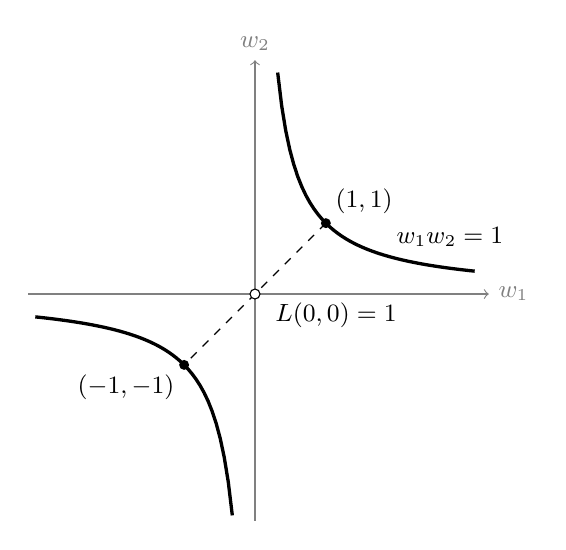
\begin{tikzpicture}[scale=0.9,font=\small]
  \draw[->,gray] (-3.2,0) -- (3.3,0) node[right] {$w_1$};
  \draw[->,gray] (0,-3.2) -- (0,3.3) node[above] {$w_2$};
  \draw[very thick,domain=0.32:3.1,samples=50] plot (\x,{1/\x});
  \draw[very thick,domain=-3.1:-0.32,samples=50] plot (\x,{1/\x});
  \fill (1,1) circle (2pt) node[above right] {$(1,1)$};
  \fill (-1,-1) circle (2pt) node[below left] {$(-1,-1)$};
  \draw[dashed] (1,1) -- (-1,-1);
  \draw[fill=white] (0,0) circle (2pt);
  \node[right] at (0.15,-0.3) {$L(0,0)=1$};
  \node at (2.75,0.8) {$w_1w_2=1$};
\end{tikzpicture}
\caption{Mínimos globales de $L(w_1,w_2)=(1-w_1w_2)^{2}$ (\cref{ej:red-lineal}). El segmento que une dos mínimos sale del conjunto de mínimos: la pérdida no es convexa.}
\label{fig:hiperbola}
\end{figure}

\begin{observacion}[Conexión con los LLM]
La pérdida de un Transformer como función de sus pesos no es convexa, y no hay garantía teórica general de que el descenso de gradiente alcance un mínimo global. En la práctica, el entrenamiento funciona de manera muy robusta gracias a la sobreparametrización, la inicialización cuidadosa, la normalización y los métodos adaptativos (módulos~7 y~11). La explicación teórica completa de este hecho sigue siendo un problema abierto.
\end{observacion}

\begin{lecturas}
\item Boyd y Vandenberghe~\cite{bv}, §3.1 «Basic properties and examples» (definición, condiciones de primer y segundo orden, ejemplos, incluida log-suma-exp), §3.2 «Operations that preserve convexity» y §4.2 «Convex optimization» (óptimos locales y globales).
\item Stanford EE364a~\cite{ee364a}, transparencias «Convex functions».
\item Goodfellow, Bengio y Courville~\cite{gbc}, §4.3 (optimización convexa frente a no convexa).
\end{lecturas}

\section*{Ejercicios del tema 5}
\addcontentsline{toc}{section}{Ejercicios del tema 5}

\begin{ejercicio}{1}{eje:5-vf}
Justifique si son verdaderas o falsas: (a) toda función $C^{2}$ con hessiano semidefinido positivo en todo $\R^{n}$ es convexa; (b) el producto de dos funciones convexas es convexo; (c) el máximo de dos funciones convexas es convexo.
\end{ejercicio}

\begin{ejercicio}{2}{eje:5-hessianos}
Decida, con el \cref{teo:segundo-orden}, cuáles de las siguientes funciones de $\R^{2}$ son convexas y cuáles estrictamente convexas: (a) $x^{2}+xy+y^{2}$; (b) $x^{2}-4xy+y^{2}$; (c) $e^{x+y}$; (d) $x^{4}+y^{2}$.
\end{ejercicio}

\begin{ejercicio}{2}{eje:5-boyd}
En el dominio $\R^{2}_{++}=\{(x_1,x_2):x_1>0,\ x_2>0\}$, determine si cada función es convexa, cóncava o ninguna de las dos: (a) $f(x)=x_1x_2$; (b) $f(x)=1/(x_1x_2)$; (c) $f(x)=x_1^{2}/x_2$.
\fuente{adaptado de Boyd y Vandenberghe~\cite{bv}, ejercicio~3.16 (selección de casos; se omite el estudio de la cuasiconvexidad).}
\end{ejercicio}

\begin{ejercicio}{2}{eje:5-red}
Sea $L(w_1,w_2)=(2-w_1w_2)^{2}$, la pérdida de una red lineal de dos capas con el dato $(x,y)=(1,2)$. (a) Compruebe que $(1,2)$ y $(2,1)$ son mínimos globales y evalúe $L$ en su punto medio. (b) Calcule $H_L(0,0)$ y clasifique el origen. (c) Concluya sobre la convexidad de $L$.
\end{ejercicio}

\begin{ejercicio}{3}{eje:5-softmax-W}
Demuestre directamente, a partir de la \cref{def:convexa} y de la convexidad de $\varphi(z)=-z_c+\LSE(z)$, que $L(W)=\varphi(Wx)$ es convexa en $W$ para $x$ fijo. Explique qué paso de la demostración falla para una red $\varphi(W_2\,\sigma(W_1x))$ con una función de activación no lineal $\sigma$.
\end{ejercicio}

\begin{ejercicio}{3}{eje:5-unico}
Sea $f\colon C\to\R$ estrictamente convexa. Demuestre que $f$ tiene a lo sumo un mínimo global. Demuestre que la entropía cruzada $L(z)$ no es estrictamente convexa en $\R^{K}$. Demuestre que $L_\mu(z)=L(z)+\tfrac{\mu}{2}\norm{z}^{2}$, con $\mu>0$, es estrictamente convexa, que tiene a lo sumo un mínimo y que, si lo tiene, sus componentes suman cero.
\end{ejercicio}
